% В этом файле следует писать текст работы, разбивая его на
% разделы (section), подразделы (subsection) и, если нужно,
% главы (chapter).

% Предварительно следует указать необходимую информацию
% в файле SETUP.tex

%% В этот файл не предполагается вносить изменения

% В этом файле следует указать информацию о себе
% и выполняемой работе.

\documentclass [fontsize=14pt, paper=a4, pagesize, DIV=calc]%
{scrartcl}
% ВНИМАНИЕ! Для использования глав поменять
% scrartcl на scrreprt

% Здесь ничего не менять
\usepackage [T2A] {fontenc}   % Кириллица в PDF файле
\usepackage [utf8] {inputenc} % Кодировка текста: utf-8
\usepackage [russian] {babel} % Переносы, лигатуры

%%%%%%%%%%%%%%%%%%%%%%%%%%%%%%%%%%%%%%%%%%%%%%%%%%%%%%%%%%%%%%%%%%%%%%%%
% Создание макроса управления элементами, специфичными
% для вида работы (курс., бак., маг.)
% Здесь ничего не менять:
\usepackage{ifthen}
\newcounter{worktype}
\newcommand{\typeOfWork}[1]
{
	\setcounter{worktype}{#1}
}

% ВНИМАНИЕ!
% Укажите тип работы: 0 - курсовая, 1 - бак., 2 - маг.,
% 3 - бакалаврская с главами.
\typeOfWork{1}
% Считается, что курсовая и бак. бьются на разделы (section) и
% подразделы (subsection), а маг. — на главы (chapter), разделы и
%  подразделы. Если хочется,
% чтобы бак. была с главами (например, если она большая),
% надо выбрать опцию 3.

% Если при выборе 2 или 3 вы забудете поменять класс
% документа на scrreprt (см. выше, в самом начале),
% то получите ошибку:
% ./aux/appearance.tex:52: Package scrbase Error: unknown option ` chapterprefix=

%%%%%%%%%%%%%%%%%%%%%%%%%%%%%%%%%%%%%%%%%%%%%%%%%%%%%%%%%%%%%%%%%%%%%%%%
% Информация об авторе и работе для титульной страницы

\usepackage {titling}

% Имя автора в именительном падеже (для маг.)
\newcommand {\me}{%
А.\,С.~Коненко
}

% Имя автора в родительном падеже (для курсовой и бак.)
\newcommand {\byme}{%
А.\,С.~Коненко%
}

% Научный руководитель
\newcommand{\supervisor}%
{к.ф.-м.н., старший преподаватель Р. Б. Штейнберг}

% идентифицируем пол (только для курсовой и бак.)
\newcommand{\bystudent}{
Студента %Студентки
}

% Год публикации
\date{2015}

% Название работы
\title{Оптимизация работы анализа псевдонимов в ОРС}

% Кафедра
%

\newcommand {\direction} {%
Направление подготовки\\02.\ifthenelse{\value{worktype} = 2}{04}{03}.02 ---
Фундаментальная информатика\\и информационные технологии%
}

%%%%%%%%%%%%%%%%%%%%%%%%%%%%%%%%%%%%%%%%%%%%%%%%%%%%%%%%%%%%%%%%%%%%%%%%
% Другие настраиваемые элементы текста

% Листинги с исходным кодом программ: укажите язык программирования
\usepackage{listings}
\lstset{
    language=[ISO]C++,%  Язык указать здесь
    basicstyle=\small\ttfamily,
    breaklines=true,%
    showstringspaces=false%
    inputencoding=utf8x%
}
% полный список языков, поддерживаемых данным пакетом, есть,
% например, здесь (стр. 13):
% ftp://ftp.tex.ac.uk/tex-archive/macros/latex/contrib/listings/listings.pdf

% Гиперссылки: настройте внешний вид ссылок
\usepackage%
[pdftex,unicode,pdfborder=0,draft=false,%backref=page,
    hidelinks, % убрать, если хочется видеть ссылки: это
               % удобно в PDF файле, но не должно появиться на печати
    bookmarks=true,bookmarksnumbered=false,bookmarksopen=false]%
{hyperref}

\usepackage {amsmath}      % Больше математики
\usepackage {amssymb}
\usepackage {textcase}     % Преобразование к верхнему регистру
\usepackage {indentfirst}  % Красная строка первого абзаца в разделе

\usepackage {fancyvrb}     % Листинги: определяем своё окружение Verb
\DefineVerbatimEnvironment% с уменьшенным шрифтом
	{Verb}{Verbatim}
	{fontsize=\small}

% Вставка рисунков
\usepackage {graphicx}

% Общее оформление
% ----------------------------------------------------------------
% Настройка внешнего вида

%%% Шрифты

% если закомментировать всё — консервативная гарнитура Computer Modern
\usepackage{paratype} % профессиональные свободные шрифты
%\usepackage {droid}  % неплохие свободные шрифты от Google
%\usepackage{mathptmx}
%\usepackage {mmasym}
%\usepackage {psfonts}
%\usepackage{lmodern}
%var1: lh additions for bold concrete fonts
%\usepackage{lh-t2axccr}
%var2: the package below could be covered with fd-files
%\usepackage{lh-t2accr}
%\usepackage {pscyr}

% Геометрия текста

\usepackage{setspace}       % Межстрочный интервал
\onehalfspacing

\newlength\MyIndent
\setlength\MyIndent{1.25cm}
\setlength{\parindent}{\MyIndent} % Абзацный отступ
\frenchspacing            % Отключение лишних отступов после точек
\KOMAoptions{%
    DIV=calc,         % Пересчёт геометрии
    numbers=endperiod % точки после номеров разделов
}

                            % Консервативный вариант:
%\usepackage                % ручное задание геометрии
%[%                         % (не рекомендуется в проф. типографии)
%  margin = 2.5cm,
  %includefoot,
  %footskip = 1cm
%] %
%  {geometry}

%%% Заголовки



\ifthenelse{\equal{\theworktype}{2}}{%
\KOMAoptions{%
    numbers=endperiod,% точки после номеров разделов
    headings=normal,   % размеры заголовков поменьше стандартных
    chapterprefix=true,% Печатать слово Глава в магистерской
    appendixprefix=true% Печатать слово Приложение
}
}

% шрифт для оформления глав и названия содержания
\newcommand{\SuperFont}{\Large\sffamily\bfseries}

% Заголовок главы
\ifthenelse{\value{worktype} > 1}{%
\renewcommand{\SuperFont}{\Large\normalfont\sffamily}
\newcommand{\CentSuperFont}{\centering\SuperFont}
\usepackage{fncychap}
\ChNameVar{\SuperFont}
\ChNumVar{\CentSuperFont}
\ChTitleVar{\CentSuperFont}
\ChNameUpperCase
\ChTitleUpperCase
}

% Заголовок (под)раздела с абзацного отступа
\addtokomafont{sectioning}{\hspace{\MyIndent}}

\renewcommand*{\captionformat}{~---~}
\renewcommand*{\figureformat}{Рисунок~\thefigure}

%%% Оглавление
\usepackage{tocloft}

% шрифт и положение заголовка
\ifthenelse{\value{worktype} > 1}{%
\renewcommand{\cfttoctitlefont}{\hfil\SuperFont\MakeUppercase}
}{
\renewcommand{\cfttoctitlefont}{\hfil\SuperFont}
}

% слово Глава
\usepackage{calc}
\ifthenelse{\value{worktype} > 1}{%
\renewcommand{\cftchappresnum}{Глава }
\addtolength{\cftchapnumwidth}{\widthof{Глава }}
}

% Очищаем оформление названий старших элементов в оглавлении
\ifthenelse{\value{worktype} > 1}{%
\renewcommand{\cftchapfont}{}
\renewcommand{\cftchappagefont}{}
}{
\renewcommand{\cftsecfont}{}
\renewcommand{\cftsecpagefont}{}
}

\ifthenelse{\value{worktype} > 1}{%
    \renewcommand{\cftchapaftersnum}{.}
}{
\renewcommand{\cftsecaftersnum}{.}
\renewcommand{\cftsubsecaftersnum}{.}
}
%%% Списки (enumitem)

\usepackage {enumitem}      % Списки с настройкой отступов
\setlist %
{ %
  leftmargin = \parindent, itemsep=.5ex, topsep=.4ex
} %

% По ГОСТу нумерация должны быть буквами: а, б...
%\makeatletter
%    \AddEnumerateCounter{\asbuk}{\@asbuk}{м)}
%\makeatother
%\renewcommand{\labelenumi}{\asbuk{enumi})}
%\renewcommand{\labelenumii}{\arabic{enumii})}

%%% Таблицы: выбрать более подходящие

\usepackage{booktabs} % считаются наиболее профессионально выполненными
%\usepackage{ltablex}
%\newcolumntype {L} {>{---}l}

%%% Библиография

\usepackage{csquotes}        % Оформление списка литературы
\usepackage[
  backend=biber,
  hyperref=auto,
  language=auto,
  citestyle=gost-numeric,
  bibstyle=gost-numeric,
]{biblatex}
\addbibresource{biblio.bib} % Файл с лит.источниками

% Настройка величины отступа в списке
\ifthenelse{\value{worktype} < 2}{%
\defbibenvironment{bibliography}
  {\list
     {\printtext[labelnumberwidth]{%
    \printfield{prefixnumber}%
    \printfield{labelnumber}}}
     {\setlength{\labelwidth}{\labelnumberwidth}%
      \setlength{\leftmargin}{\labelwidth}%
      \setlength{\labelsep}{\dimexpr\MyIndent-\labelwidth\relax}% <----- default is \biblabelsep
      \addtolength{\leftmargin}{\labelsep}%
      \setlength{\itemsep}{\bibitemsep}%
      \setlength{\parsep}{\bibparsep}}%
      \renewcommand*{\makelabel}[1]{\hss##1}}
  {\endlist}
  {\item}
}{}

% ----------------------------------------------------------------
% Настройка переносов и разрывов страниц

\binoppenalty = 10000      % Запрет переносов строк в формулах
\relpenalty = 10000        %

\sloppy                    % Не выходить за границы бокса
%\tolerance = 400          % или более точно
\clubpenalty = 10000       % Запрет разрывов страниц после первой
\widowpenalty = 10000      % и перед предпоследней строкой абзаца

% ----------------------------

% Стили для окружений типа Определение, Теорема...
% ���������� ������ (ntheorem)

\usepackage [thmmarks, amsmath] {ntheorem}
\theorempreskipamount 0.6cm

\theoremstyle {plain} %
\theoremheaderfont {\normalfont \bfseries} %
\theorembodyfont {\slshape} %
\theoremsymbol {\ensuremath {_\Box}} %
\theoremseparator {:} %
\newtheorem {mystatement} {�����������} [section] %
\newtheorem {mylemma} {�����} [section] %
\newtheorem {mycorollary} {���������} [section] %

\theoremstyle {nonumberplain} %
\theoremseparator {.} %
\theoremsymbol {\ensuremath {_\diamondsuit}} %
\newtheorem {mydefinition} {�����������} %

\theoremstyle {plain} %
\theoremheaderfont {\normalfont \bfseries} 
\theorembodyfont {\normalfont} 
%\theoremsymbol {\ensuremath {_\Box}} %
\theoremseparator {.} %
\newtheorem {mytask} {������} [section]%
\renewcommand{\themytask}{\arabic{mytask}}

\theoremheaderfont {\scshape} %
\theorembodyfont {\upshape} %
\theoremstyle {nonumberplain} %
\theoremseparator {} %
\theoremsymbol {\rule {1ex} {1ex}} %
\newtheorem {myproof} {��������������} %

\theorembodyfont {\upshape} %
%\theoremindent 0.5cm
\theoremstyle {nonumberbreak} \theoremseparator {\\} %
\theoremsymbol {\ensuremath {\ast}} %
\newtheorem {myexample} {������} %
\newtheorem {myexamples} {�������} %

\theoremheaderfont {\itshape} %
\theorembodyfont {\upshape} %
\theoremstyle {nonumberplain} %
\theoremseparator {:} %
\theoremsymbol {\ensuremath {_\triangle}} %
\newtheorem {myremark} {���������} %
\theoremstyle {nonumberbreak} %
\newtheorem {myremarks} {���������} %

% Титульный лист
% Макросы настройки титульной страницы
% В этот файл не предполагается вносить изменения

%\usepackage {showframe}

% Вертикальные отступы на титульной странице
\newcommand{\vgap}{\vspace{10pt}}
% \newcommand{\vgap}{\vspace{16pt}}

% Помещение города и даты в нижний колонтитул
\usepackage{scrlayer}
\DeclareNewLayer[
  foot,
  foreground,
  contents={%
    \raisebox{\dp\strutbox}[\layerheight][0pt]{%
      \parbox[b]{\layerwidth}{\centering Ростов-на-Дону\\ \thedate%
       \\\mbox{}
       }}%
  }
]{titlepage.foot.fg}
\DeclareNewPageStyleByLayers{titlepage}{titlepage.foot.fg}


\AtBeginDocument %
{ %
  %
  \begin{titlepage}
  %
    \thispagestyle{titlepage}

    {\centering
    %
    \MakeTextUppercase {МИНИСТЕРСТВО ОБРАЗОВАНИЯ И НАУКИ РФ}

    \vgap

    Федеральное государственное автономное образовательное\\
    учреждение высшего образования\\
    \MakeTextUppercase {Южный федеральный университет}

    \vgap

	Институт математики, механики и компьютерных наук
    имени~И.\,И.\,Воровича

    \vgap

    \direction

    \vspace* {\fill}

    \ifthenelse{\value{worktype} = 2}{%
    \me

    \vgap}{}

    \MakeTextUppercase{\thetitle}

    \ifthenelse{\value{worktype} = 2}{%
     \vgap

    Магистерская диссертация}{}
    \ifthenelse{\value{worktype} = 0}{
     \vgap

    Курсовая работа
    }{}%
    \ifthenelse{\value{worktype} = 1 \OR \value{worktype} = 3}{
     \vgap

    Выпускная квалификационная работа\\
    на степень бакалавра
    }{}%

    \vspace {\fill}

    \begin{flushright}
    \ifthenelse{\value{worktype} = 1 \OR \value{worktype} = 0}{
      \bystudent \ifthenelse{\value{worktype} = 0}{3}{4}\ курса\\
      \byme
    }{}

    \vgap

    Научный руководитель:\\
    \supervisor\\
    \ifthenelse{\value{worktype} = 2}{%
    Рецензент:\\
    ученая степень, ученое звание [, должность]
    И. О. Фамилия
    }{}
	\end{flushright}
\ifthenelse{\value{worktype} = 0}{
\vspace{\fill}
        \begin{flushleft}
          \begin{tabular}{cc}
            \underline{\hspace{4cm}}&\underline{\hspace{5cm}}\\
            {\small оценка (рейтинг)} & {\small  подпись руководителя}\\
          \end{tabular}
          \\[1cm]
%          Утверждаю:\\руководитель направления ФИИТ \underline{\hspace{4cm}}
%В.\,С.\,Пилиди
        \end{flushleft}
}{}
\ifthenelse{\value{worktype} = 1 \OR \value{worktype} = 3}{
\vspace{\fill}
        \begin{flushleft}
Допущено к защите:\\руководитель направления ФИИТ
\underline{\hspace{4cm}}
В.\,С.\,Пилиди
        \end{flushleft}
}{}


  	\vspace {\fill}

  %Ростов-на-Дону

    %\thedate

  }\end{titlepage}
  %
  %
  \tableofcontents
  %
  \clearpage
} %


% Команды для использования в тексте работы
% макросы для начала введения и заключения
\newcommand{\Intro}{\addsec{Введение}}
\ifthenelse{\value{worktype} > 1}{%
    \renewcommand{\Intro}{\addchap{Введение}}%
}

\newcommand{\Conc}{\addsec{Заключение}}
\ifthenelse{\value{worktype} > 1}{%
    \renewcommand{\Conc}{\addchap{Заключение}}%
}

% Правильные значки для нестрогих неравенств и пустого множества
\renewcommand {\le} {\leqslant}
\renewcommand {\ge} {\geqslant}
\renewcommand {\emptyset} {\varnothing}

% N ажурное: натуральные числа
\newcommand {\N} {\ensuremath{\mathbb N}}

% значок С++ — используйте команду \cpp
\newcommand{\cpp}{C\nolinebreak\hspace{-.05em}%
\raisebox{.2ex}{+}\nolinebreak\hspace{-.10em}%
\raisebox{.2ex}{+}}

% Неразрывный дефис, который допускает перенос внутри слов,
% типа жёлто-синий: нужно писать жёлто"/синий.
\makeatletter
    \defineshorthand[russian]{"/}{\mbox{-}\bbl@allowhyphens}
\makeatother

\endinput

% Конец файла


\begin{document}

\Intro

% Задачей настоящей бакалаврской работы является исследование темы анализа псевдонимов и оптимизация работы анализа псевдонимов в ОРС - исследовательском оптимизирующем компиляторе языков Си и Фортран.

\begin{mydefinition}
Анализ псевдонимов -- это комплекс алгоритмов, работающих в компиляторе, который позволяет получать информацию о ряде важных взаимоотношений между ячейками памяти и указателями на них.
\end{mydefinition}

Информация получаемая анализом псевдонимов необходима для ряда применений:
\begin{itemize}
\item уточнения некоторых других анализов кода -- тех, которые в своей работе опираются на взаимоотношения между данными~\autocite{Voevodin}.
\item проверки предусловий применимости некоторых преобразований кода:  некоторые преобразования невозможно сделать при псевдонимной связи между данными в блоке, а некоторые, наоборот, в своей работы опираются на наличие таких связей.
\item для статических проверок программы на возможные ошибки.
\end{itemize}

\begin{myexampless}
В качестве примера анализа, который может уточнить свои результаты за счет анализа псевдонимов, можно привести анализ вычисляющий объем памяти необходимой для работы некоторому блоку кода. Во время его работы полезно знать, что какие-то из переменных в заданном блоке -- псевдонимы.

В качестве примера преобразования, которому необходима информация о превдонимах можно привести раскрутку цикла, которой необходимо, чтобы счетчик цикла не менялся в его теле.

Возможной ошибкой, которую может обнаружить анализ псевдонимов, может быть ситуация, когда в функции две переменные всюду друг другу псевдонимы.
\end{myexampless}

\begin{mydefinition}
Два указателя a и b будем называть псевдонимами, если они указывают на одну и ту же область памяти. Причем мы можем говорить об этом отношении с некоторой уверенностью, если анализ делает упрощения и пренебрежения точностью для ускорения работы и уменьшения потребления памяти, к примеру -- игнорирует контекст вызова процедур.
\end{mydefinition}

\begin{mydefinition}
Контекстом вызова процедуры при анализе псевдонимов мы будем называть информацию о взаимоотношении между всеми ячейками памяти и всеми указателями, которые находятся в области видимости данной процедуры при вызове её из данного места какой-то процедуры. 
\end{mydefinition}

Целью анализа псевдонимов является статическое (на этапе компиляции) определение для каждой пары указателей и, возможно, контекстов вызова функции, как соотносятся области памяти на которые указывают эти указатели. Всего выделяют четыре взаимоотношения между указателями:
\begin{description}
  \item[MustAlias] Указатели точно указывают в одну область памяти, т.е. являются псевдонимами.
  \item[PartialAlias] Объекты, на которые они указывают пересекаются в памяти, но начинаются не с одного адреса.
  \item[MayAlias] Указатели могут указывать в одну область памяти.
  \item[NoAlias] Указатели точно указывают в разные области памяти.
\end{description}

\begin{ListingEnv}[H]
\begin{lstlisting}
int* f(int* a, int* X)
{
    int* p;
    int i;
    ...
    for (i=0; i < 8; ++i)
    {
        X[i] = g(a, p);
    }
    ...
    return p;
}
\end{lstlisting}
\caption{Пример функции переданной для анализа}
\end{ListingEnv}

Для примера рассмотрим функцию приведенную в листинге 0.1. Небольшое число число итерации цикла может навести на мысль развернуть цикл, но это будет эквивалентным преобразрованием, только если $a$, $p$ и $X$ точно не являются псевдонимами к $i$, т.е. в теле цикла счетчик цикла не может изменится. Как видно, информация получаемая этим анализом может предостеречь компилятор от преобразований, которые могут сделать программу не эквивалентной исходной.

\begin{myremark}
Следует учитывать, что анализ псевдонимов исходит из того, что код программы не содержит элементов, которые могут привести к неопределенному поведению, т.е. таких элементов, например, как обращения к элементам находящимся за границами массивов. В примере выше компилятору будет достаточно убедится, что нигде в функции не берется адрес переменной $i$ и попытка выполнения, например, $p = \&p + 1$ (исходя из предположения, что переменные $i$ и $p$ соседи на стеке и лежат там именно в этом порядке) будет пропущена как потенциальное создание псевдонима.
\end{myremark}

%\subsection{Классификация анализов псевдонимов}

Существует ряд классификаций анализов псевдонимов. Ниже приведены ключевые, которые, в частности, затрагивались в докладе~\autocite{GohmanAAinLLVM} одного из разработчиков LLVM.

\begin{mydefinition}
Анализ называют чувствительным к контексту -- $context$-$sensitive$, если он различает вызовы анализируемой функции с различными взаимоотношениями в смысле псевдонимов между указателями находящимися в области видимости и опираясь на контекст построить результат с наибольшей возможной уверенностью об отношении. В обратном случае, если для процедуры строится один контекстно-независимый результат, который верен для любого контекста вызова, но пессимистичен, т.е. содержит много $MayAlias$ результатов, анализ называют не чувствительным к контексту -- $context$-$insensitive$.
\end{mydefinition}

\begin{mydefinition}
Анализ называют $flow$-$sensitive$, если он чувствителен к местам вхождений переданных указателей при ответе на запросы по результату анализа, иначе он является $flow$-$insensitive$, т.е. имеющим представление только о конечном взаимоотношении между этими указателями, но не имеющим промежуточных результатов.
\end{mydefinition}

\begin{mydefinition}
Анализ называют чувствительным к полям структур -- $field$-$sensitive$, если он способен различать поля структур при анализе. В обратном случае, если псевдонимом к чему-либо является какой-то член структуры, а анализ объявляет псевдонимом всё структуру целиком, то анализ называется нечувствительным к полям структур -- $field$-$insensitive$.
\end{mydefinition}

\begin{mydefinition}
Если анализ строится для языков в которых отсутствуют сырые указатели и есть сильная система типов вроде Haskell или Java, то его строят на основе анализа типов и называют $type$-$based$. Если же анализ строится для языка, в котором есть сырые указатели и преобразования типов, вроде языков С/С++, то анализ строят на анализе потока управления программы и такой анализ называют $flow$-$based$.
\end{mydefinition}

%--------------------------------------------------------------------------------------------------------------------
\section{Анализ существующих подходов к анализу псевдонимов}

В ходе работы был изучен ряд подходов к анализу псевдонимов. В основном это были алгоритмы реализованные в LLVM. 

$BasicAA$ -- Один из базовых анализов применяемых в LLVM и производящий по заявлениям документации~\autocite{LLVMAAI} агрессивный локальный анализ и исходящий, в частности из следующих предположений:
\begin{itemize}
\item Глобальные переменные, память выделенная на стеке и в динамической памяти никогда не пересекается.
\item Различные поля структуры никогда не псевдонимы друг другу.
\item Большинство функций страндартной библиотеки Си не обращаются к памяти или только читают её.
\item Вызовы функций не могут модифицировать или ссылатся на части стека, которая выделена не для них.
\end{itemize}

$Steensgaard’s algorithm$ -- межпроцедурный анализ с хорошей скоростью работы, но с большим числом упрощений и обобщений. Он принадлежит к классу $unification$-$based$, т.е. его работа основа на присваении классов переменным и их объединении на основе анализа программы. Из его описания в заметке ~\autocite{SteensgaardsNote} можно понять его сильные и слабые стороны. Его реализация так же используется в LLVM в местах, где скорость работы важнее её точности. Принцип работы изображен на рисунке ~\ref{fig:steensgaard}.

\begin{figure}[H]
\centering
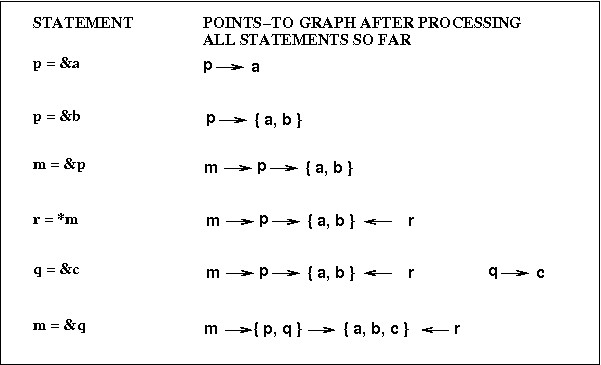
\includegraphics[width=0.9\textwidth]{img/steensgaard.jpg}
\caption{\label{fig:steensgaard} Демонстрация принципа работы алгоритма Стинсгарда}
\end{figure}

Так же были изучены работы Моники Лэм и Роберта Уилсона, в которых рассматривался такой подход к межпроцедурному анализу, как частично трансферные функции, который предлагает во время анализа функций строить отображения из контекста вызова в контекст, получаемый на выходе, что должно ускорять межпроцедурный анализ, отсекая повторные анализы вызовов функций не только с одним и тем же контекстом, но и подобными ему.

При существовании в компиляторе нескольких реализаций анализа псевдонимов часто прибегают к их последовательному применению по цепочке, запуская более тяжеловесные алгоритмы для уточнения только критичных участков. Такой принцип, например, принят в инфраструктуре LLVM.

%--------------------------------------------------------------------------------------------------------------------
\section{Существующая реализация анализа в ОРС}

Оптимизирующая распараллеливающая система разрабатываемая на мехмате является экспериментальным исследовательским проектом, целью которого является изучение методов автоматической оптимизации программ. Как и прочие компиляторы выполняющие в процессе своей работы анализ и преобразования программ, компилятор ОРС имеет в своём составе реализацию анализа псевдонимов.

Пользуясь описанной классификацией анализов существующую в ОРС реализацию можно описать как $flow$-$based$, $context$-$sensitive$, $flow$-$sensitive$, $field$-$sensitive$ (по умолчанию. Может быть и $field$-$insensitive$) анализ псевдонимов.

Существующая реализация достаточно точная, но весьма медленная и требует сравнительно большой объем памяти. Принцип её работы заключается в осуществлении для каждой функции обхода всех путей от входа до выхода в факторизованном графе потока управления с накоплением результатов анализа и анализе вызванной функции для каждого контекста отдельно. Такой подход позволяет строить достаточно точный анализ, так как по сути представляет собой практически полноценное выполнение всех функций.

Как и многие другие части компилятора ОРС модуль анализа псевдонимов имеет два набора тестов:
\begin{enumerate}
    \item Тесты производительности.
    \item Тесты корректности.
\end{enumerate}

Для тестирования производительности используются бенчмарки, являющиеся по сути исходными кодами реальных программ или их частей, которые подаются на вход компилятору и производится профилирование процесса выполнения. Например, одним из бенчмарков является $quagga$ -- пакет реализующий протоколы динамической маршрутизации используемый в UNIX подобных операционных системах.
% откуда взялись бенчмарки и почему было принято решение тестировать анализ с их помощью (это реальные программы)

При разработке ОРС используется модульное тестирование, которое помогает команде разрабочиков контролировать корректность работы компилятора и избегать случайной поломки частей компилятора.
% модульное тестирование.

Для упрощения работы с результатом работы анализа псевдонимов, в ОРС используется построение графа зависимостей.
% деп.граф, анализ зависимостей. Основная масса анализов и преобразований используют АА через деп.граф.

\section{Ускорение анализа}

В существующем анализе посредством профилирования, чтения кода и документации было обнаружено два перспективных направления, переработка которых могла принести хорошие результаты, а именно за счет незначительного ухудшения качества увеличить скорость работы анализа. А именно:

В процедурной части анализа, в случаях, когда в функции имеется множество расходящихся и сразу же сходящихся веток, что свойственно, например, графовым алгоритмам, полный обход всех путей от входа до выхода занимает значительное время.

Для решения этой проблемы была предпринята попытка применить некоторые идеи из алгоритма Стинсгарда и изменить логика обхода графа управления в сторону раннего слияния результатов анализа. Для этого в местах ветвления анализ пытается заглянуть вперед для нахождения ближайшего общего потомка веток для объединения в нём результатов анализа, а не в конце программы. Эта модификация незначительно ухудшив результаты анализа (находилось больше псевдонимов) привела с ускорению анализа подобных функций, но существуют примеры, на которых анализ существенно замедлился. В листинге 3.1 приведена схема функции, анализ которой хорошо ускорился за счет данной модификации.

\begin{ListingEnv}[H]
\begin{lstlisting}
void f(int* a, int* b)
{
    if (...)
    {
        ...
    }
    else
    {
        ...
    }
    ...
    if (...)
    {
        ...
    }
    else
    {
        ...
    }
    ...
}
\end{lstlisting}
\caption{Общий вид функций, анализ которых ускоряется за счет раннего слияния результатов обхода ветвей графа управления}
\label{list:otherlevels}
\end{ListingEnv}

В межпроцедурной части анализа существующий алгоритм производит детальный анализ для каждого места вызова функции, что оказывается излишним в случае, если контекст вызовов не меняется.

Для решения второй проблемы первой идеей было воспользоватся наработками описанными в работе Лэм и Вильсона~\autocite{WilsonLamSIGPLAN95} и анализировать контексты для которых выполняются проверки, чтобы в случае вызова в подобных контекстах выполнять анализ однократно. Но полноценная реализация построения частично трансферных функций имела значительную трудоёмкость, поэтому было принято решение сначала, для проверки гипотезы, реализовать простое кэширование результата для одних и тех же контекстов вызова функции. Этот подход дал неплохие результаты: тестов небольших размеров скорость построения результата анализа почти не изменилась, но на достаточно сложных бенчмарках, с большим числом вызывающих друг друга функций скорость удвоилась.

\Conc

В таблице 1 представлены результаты тестирования скорости построения результата анализа для исходного алгоритма, двух созданных модификаций и их комбинации. Числа в клетках - среднее время в миллисекундах, которое потребовалось на построение результата анализа для соответствующего бенчмарка на 20 запусках.

Сборка проекта осуществлялась g++ 4.9.2 на Ubuntu 15.04. Компьютер на котором осуществлялось тестирование имеет процессор Intel(R) Core(TM) i7-4700MQ с тактовой частотой 2.4 GHz и автоматическим её увеличением до 3.4 GHz. Так как алгоритмы анализа работают в одном потоке, частота процессора играет большую роль, чем число ядер.

\begin{table}[h!]
\label{tabl:Profiling}
\begin{tabular}{l | c | c | c | c }
Бенчмарк & Исходная реализация & Слияние & Кэширование & Оба \\
\hline \hline
linpack & 193 & 189 & 184 & 183 \\
md & 46 & 44 & 40 & 40\\ 
whetstone & 81 & 78 & 75 & 76\\
smith & 211 & 117 & 98 & 97\\
revrina & 191 & 192 & 67 & 68\\
lbm & 446 & 4474 & 341 & 4490\\
hirschberg & 604 & 570 & 309 & 306\\
hirschberg2 & 104 & 103 & 50 & 51\\
quagga & 23 & 6 & 22 & 6
\end{tabular}
\caption{Результаты тестирования}
\end{table}

\newpage % Почему-то библиография накладывалась на таблицу. Быть не должно этого тут.

% Печать списка литературы (библиографии)
\printbibliography[
    heading=bibintoc%
    ,title=Библиография % если хочется это слово
]
% Файл со списком литературы: biblio.bib
% Подробно по оформлению библиографии:
% см. документацию к пакету biblatex-gost
% http://ctan.mirrorcatalogs.com/macros/latex/exptl/biblatex-contrib/biblatex-gost/doc/biblatex-gost.pdf
% и огромное количество примеров там же:
% http://mirror.macomnet.net/pub/CTAN/macros/latex/contrib/biblatex-contrib/biblatex-gost/doc/biblatex-gost-examples.pdf

\end{document}